% LaTeX Template for short student reports.
% Citations should be in bibtex format and go in references.bib
\documentclass[a4paper, 11pt]{article}
\usepackage[top=3cm, bottom=3cm, left = 2cm, right = 2cm]{geometry} 
\geometry{a4paper} 
\usepackage[utf8]{inputenc}
\usepackage{textcomp}
\usepackage{graphicx} 
\usepackage{amsmath,amssymb}  
\usepackage{bm}  
\usepackage[pdftex,bookmarks,colorlinks,breaklinks]{hyperref}  
%\hypersetup{linkcolor=black,citecolor=black,filecolor=black,urlcolor=black} % black links, for printed output
\usepackage{memhfixc} 
\usepackage{pdfsync}  
\usepackage{fancyhdr}
\usepackage{mathpazo}
\pagestyle{fancy}

\title{COMP6257 Coursework 1}
\author{Frederik McArthur, fsm1g19@soton.ac.uk}
%\date{}

\begin{document}
\maketitle
\tableofcontents

\section{Introduction}

My project was about \ldots

I developed a system to \ldots

We did some experiments to find out \ldots

The main results were \ldots

\pagebreak

\section{Verifying the Inverse of a Partitioned Matrix}

The inverse of a partitioned matrix is given by:
$$
\begin{bmatrix}
    A & B \\
    C & D
\end{bmatrix}^{-1}
= \begin{bmatrix}
    M & -MBD^{-1} \\
    -D^{-1}CM & D^{-1} + D^{-1}CMBD^{-1}
\end{bmatrix}
    $$
Where $M = \begin{bmatrix}
    A - BD^{-1}C
\end{bmatrix}^{-1}$. To verify that $\begin{bmatrix}
    M & -MBD^{-1} \\
    -D^{-1}CM & D^{-1} + D^{-1}CMBD^{-1}
\end{bmatrix}$ is the inverse of $\begin{bmatrix}
    A & B \\
    C & D
\end{bmatrix}$, the following condition must be met:
$$
\begin{bmatrix}
    A & B \\
    C & D
\end{bmatrix} * 
\begin{bmatrix}
    M & -MBD^{-1} \\
    -D^{-1}CM & D^{-1} + D^{-1}CMBD^{-1}
\end{bmatrix}
= \begin{bmatrix}
    I & 0 \\
    0 & I
\end{bmatrix}$$
Examining each element of the matrix, and using the knowledge that $A*I = I*A = A$, and $A*A^{-1} = A^{-1}A = I$;
\begin{itemize}
    \item Row 1 Column 1;
    \begin{align*}
        AM + B(-D^{-1}CM) &= I\\
        AM - BD^{-1}CM &= I\\
        M * (A - BD^{-1}C) &= I\\
        M * M^{-1} &= I
    \end{align*}
    \item Row 1 Column 2;
    \begin{align*}
        A (-MBD^{-1}) + B(D^{-1} + D^{-1}CMBD^{-1}) &= 0 \\
        -AMBD^{-1} +BD^{-1} + BD^{-1}CMBD^{-1} &= 0\\
        (AM + I + BD^{-1}CM)BD^{-1} &= 0\\
        ((A-BD^{-1}C)M - I)BD^{-1} &= 0 \\
        (M^{-1}M - I)BD^{-1} &= 0 \\
        (I - I) BD^{-1} &= 0
    \end{align*}
    \item Row 2 Column 1;
    \begin{align*}
        CM + D(-D^{-1}CM) &= 0 \\
        CM - DD^{-1}CM &= 0 \\
        CM - ICM &= 0\\
        CM - CM &= 0
    \end{align*}
    \item and finally, Row 2 Column 2;
    \begin{align*}
        C(-MBD^{-1}) + D(D^{-1} + D^{-1}CMBD^{-1}) &= I \\
        -CMBD^{-1} +  DD^{-1} + DD^{-1}CMBD^{-1} &= I \\
        -CMBD^{-1} + I + ICMBD^{-1} &= I \\
        -CMBD^{-1} + CMBD^{-1} + I &= I \\
        I &= I
    \end{align*}
\end{itemize}
This demonstrates that $
\begin{bmatrix}
    A & B \\
    C & D
\end{bmatrix}^{-1}
= \begin{bmatrix}
    M & -MBD^{-1} \\
    -D^{-1}CM & D^{-1} + D^{-1}CMBD^{-1}
\end{bmatrix}
    $.


    
\pagebreak

\section{Bayesian Analysis of the Illustrative Polynomial}

The dataset generated for this problem was generated with Numpy, first by generating a uniform dataset, and then by applying a sinusoidal function to it. The Sklearn \verb|train_test_split| function is then used to split the dataset into both a training and a testing dataset. A plot of the training and testing dataset can be seen in Figure \ref{fig:traintestsplit}.

\begin{figure}[h]
    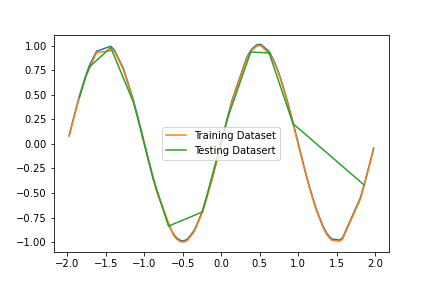
\includegraphics[width=8cm]{fig/traintestsplit.png}
    \caption{A figure showing the training and testing datasets.}
    \label{fig:traintestsplit}
\end{figure}

Polynomial regression was then performed on the data, with trials at different P values. As shown in Figure \ref{fig:pvalueboxplt} shows that as the P value increasses, the accuracy increases towards a point. Beyond a certain value, the graph will begin to overfit.

\begin{figure}[h]
    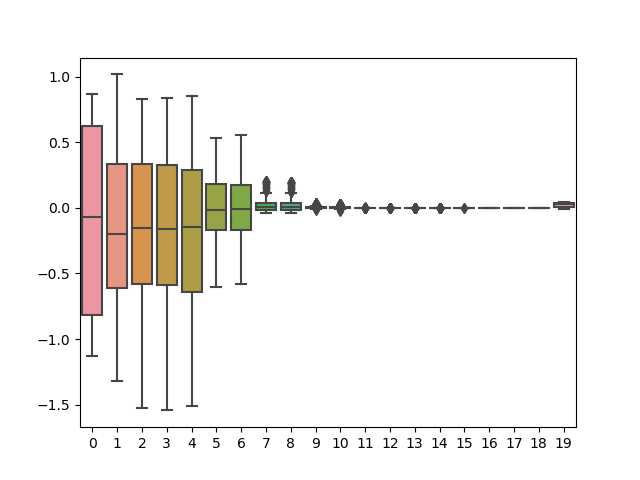
\includegraphics[width=8cm]{fig/pvalueboxplot.png}
    \caption{A figure showing the error values for different p values.}
    \label{fig:traintestsplit}
\end{figure}

\pagebreak

\section{Evaluation}

We did some experiments \ldots

\pagebreak

\section{Conclusions and Future Work}

From our experiments we can conclude that \ldots

\bibliographystyle{abbrv}
% \bibliography{references}  % need to put bibtex references in references.bib 
\end{document}